\documentclass[runningheads]{llncs}
\title{Erratum: A High-Order Discontinuous Galerkin Solver with Dynamic Adaptive Mesh Refinement to Simulate Cloud Formation Processes }
\titlerunning{A High-Order DG Solver to Simulate Cloud Formation Processes}
\author{Lukas Krenz\orcidID{0000-0001-6378-0778} \and Leonhard Rannabauer \and Michael Bader}
\authorrunning{L.\ Krenz, L.\ Rannabauer, M.\ Bader}
\institute{TUM School of Computation, Information and Technology, Technical University of Munich\\
  \email{lukas.krenz@in.tum.de}, \email{rannabau@in.tum.de}, \email{bader@in.tum.de}
} 
\usepackage[utf8]{inputenc}
%\usepackage[T1]{fontenc}
\usepackage[american]{babel}
\usepackage[autostyle, english = american]{csquotes}
% \usepackage[%
%   backend=biber,
%   url=false,
%   doi=false,
%   % style=alphabetic,
%   % backref=true,
%   % hyperref=true,
%   maxnames=3,
%   % minnames=3,
%   % maxbibnames=99,
%   firstinits=true,
%   % uniquename=init
%   ]{biblatex}
% \addbibresource{../bibliography.bib}
\usepackage{cite}
\usepackage{todonotes}


\usepackage{caption}
\usepackage{subcaption}
\usepackage{xparse} % for NewDocumentCommand
\usepackage{etoolbox} % for notblank (brackets only when argument)
\usepackage{xstring} % for \IfSubStr
\usepackage{xpatch}
\usepackage{xcolor}
\usepackage{amsmath}
\usepackage{amsfonts}
\usepackage{amssymb}
\usepackage{mathtools} % for \mathclap
\usepackage{nicefrac}
\usepackage{physics} % for derivatives
\usepackage{varioref}
\usepackage{nicefrac}
\usepackage{physics} % for derivatives
\usepackage[separate-uncertainty]{siunitx}
\usepackage{hyperref}
\usepackage[capitalise]{cleveref}
\newcommand{\creflastconjunction}{, and\nobreakspace} % use Oxford comma
\usepackage{graphicx}
\usepackage{multimedia}
%\graphicspath{{../figures/}}
\graphicspath{{.}}
\let\boundary\undefined%
\crefformat{equation}{\eqA{}Eq.~\eqB #2#1#3)}
\crefmultiformat{equation}{Eqs.~\eqMultiA#2#1#3\eqMultiB}%
{ and \eqMultiA#2#1#3\eqMultiB}{, \eqMultiA#2#1#3\eqMultiB}{ and~\eqMultiA#2#1#3\eqMultiB}
\newcommand{\eqA}{}
\newcommand{\eqB}{(}
\newcommand{\eqMultiA}{(}
\newcommand{\eqMultiB}{)}
\DeclareRobustCommand{\pcrefSingle}[1]{%
\begingroup%
  \renewcommand{\eqA}{(}\renewcommand{\eqB}{}%
\cref{#1}%
\endgroup%
}
\DeclareRobustCommand{\pcrefMulti}[1]{%
\begingroup%
    \renewcommand{\eqMultiA}{}\renewcommand{\eqMultiB}{}%
    (\cref{#1})%
\endgroup%
}
\DeclareRobustCommand{\pcref}[1]{%
\IfSubStr{#1}{,}{\pcrefMulti{#1}}{\pcrefSingle{#1}}%
}

\usepackage{bm}
% Commands/Macros
\newcommand{\muscl}{\textsc{muscl}-Hancock}
\newcommand{\dg}{\textsc{dg}}
\newcommand{\ader}{\textsc{ader}}
\newcommand{\aderdg}{\textsc{ader-dg}}
\newcommand{\amr}{\textsc{amr}}
\newcommand{\pde}{\textsc{pde}}
\newcommand{\tbb}{\textsc{tbb}}
\newcommand{\mpi}{\textsc{mpi}}

\newcommand{\softwareName}[1]{#1}
\newcommand{\exahype}{\softwareName{ExaHyPE}}
\newcommand{\exahypeengine}{\softwareName{ExaHyPE Engine}}

% Variables and other equation stuff
\newcommand{\Q}{\bm{Q}}
\newcommand{\gradQ}{\gradient{\Q}}
\newcommand{\Qrho}{\rho}
\newcommand{\Qj}{\rho \bm{v}}
\newcommand{\Qv}{\bm{v}}
\newcommand{\QE}{\rho E}
\newcommand{\potT}{\theta}
\newcommand{\backgroundPotT}{\overline{\theta}}
\newcommand{\pertubationPotT}{\theta'}
\newcommand{\stressT}{\bm{\sigma}}
\newcommand{\pressure}{p}

% Cells
\newcommand{\cell}[1][]{C_{#1}}

% Bold if no index is supplied.
\newcommand{\bmempty}[2]{
\notblank{#2}{#1}{\bm{#1}}
}

% Equation parts
\newcommand{\flux}{\bm{F}}
\newcommand{\viscFlux}{\flux^{v}}
\newcommand{\hyperFlux}{\flux^{h}}
%\newcommand{\source}{\bm{S}}
\newcommand{\source}[1][]{
  \notblank{#1}{
S_{#1}
}{
\bm{S}
}
}
\newcommand{\intdcell}[1]{\int_{\cell} #1 \dd{\bm{x}}}
\newcommand{\tv}{\operatorname{TV}}

\begin{document}
\maketitle 
%\begin{abstract}
%This is an erratum.
%In the original paper, we computed our scenarios with incorrect parameters.
%Here, we show that we get similar results with the corrected parameters.
%%\keywords{\aderdg{}  \and Navier-Stokes \and Adaptive Mesh Refinement}
%\end{abstract}
\paragraph{Background}
This is an erratum for~\cite{krenz2019high}.
When trying to reproduce our results, we noticed that we erroneously computed the cloud scenarios (in section 4.2) with different parameters as stated in the papers.
These scenarios simulate perturbations over a background state that is in hydrostatic equilibrium.
We used an incorrect background pressure of \SI{10000}{\pascal} instead of \SI{100000 }{\pascal} to compute the background states.
In our paper, we use the viscosity given by the Navier-Stokes equations to stabilize our simulations.
We stated a viscosity that is too small to ensure stable simulations with the higher background pressure.
Thus, we recomputed the key cloud scenarios with correct background pressure and modified viscosity.
All other simulation parameters are as described in~\cite{krenz2019high}.
Neither classical CFD scenarios (Taylor-Green, Lid-driven cavity, ABC-Vortex) nor the convergence test are affected.

\begin{figure}[htb]
  \begin{subfigure}[t]{0.45\columnwidth}
  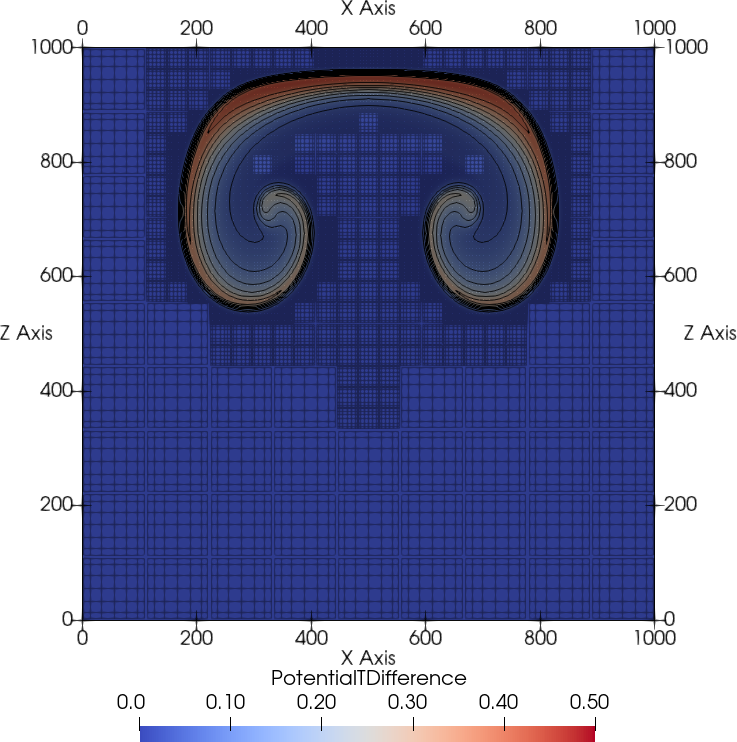
\includegraphics[width=\textwidth]{screenshots/cosine_bubble_2d_dg.png}
  \caption{\label{fig:cosine-bubble-2d-dg-amr}%
  2D Cosine bubble with AMR, computed by the ADER-DG method.
  Contours are at $-0.05, 0.05, \ldots 0.45$.
  }
  \end{subfigure}\quad
  \begin{subfigure}[t]{0.45\columnwidth}
  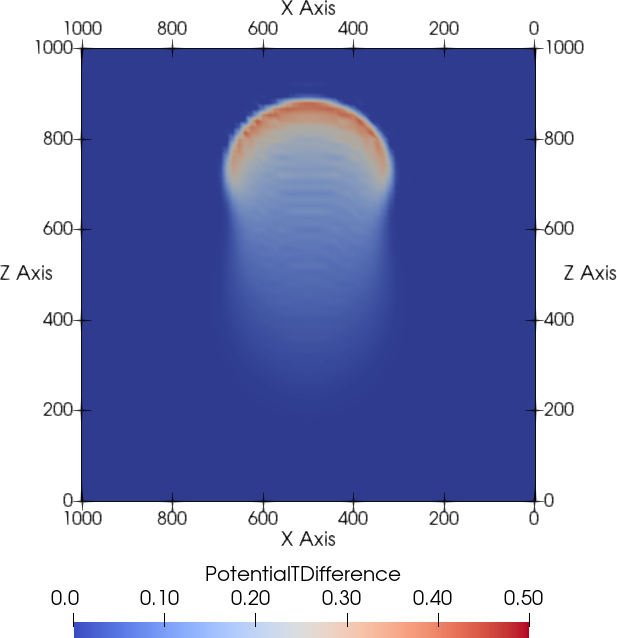
\includegraphics[width=1\textwidth]{screenshots/cosine_bubble_3d_dg.png}
  \caption{\label{fig:cosine-bubble-3d-dg-noamr}%
  3D Cosine bubble without AMR, computed by the ADER-DG method.}
  \end{subfigure}
\caption{
  Recomputed and corrected scenario to replace Figure 6 of~\cite{krenz2019high}.
}
\end{figure}
% Settings: visc 0.1, refine: 1.5, coarse: -0.5
\paragraph{Cosine Bubble (Sec. 4.2, Fig.~4 and~5 of~\cite{krenz2019high})}
We ran the cosine bubble scenario with and without adaptive mesh refinement (AMR) using the correct background pressure and a viscosity of $\mu=0.1$. 
The new result (\cref{fig:cosine-bubble-2d-dg-amr}) shows a very close agreement with the original results.
The mesh refinements for the two scenarios are not identical but of the same quality
Similar to the original results, the results obtained with a statically refined mesh are visually indistinguishable from the AMR results.
We also simulated a three-dimensional cosine bubble.
The results (\cref{fig:cosine-bubble-3d-dg-noamr}), computed with the correct background pressure and a viscosity of $\mu=0.4$, are similar to our original results.

\begin{figure}[htb] 
  \centering 
    \begin{minipage}[t]{.473\textwidth} 
    \centering
  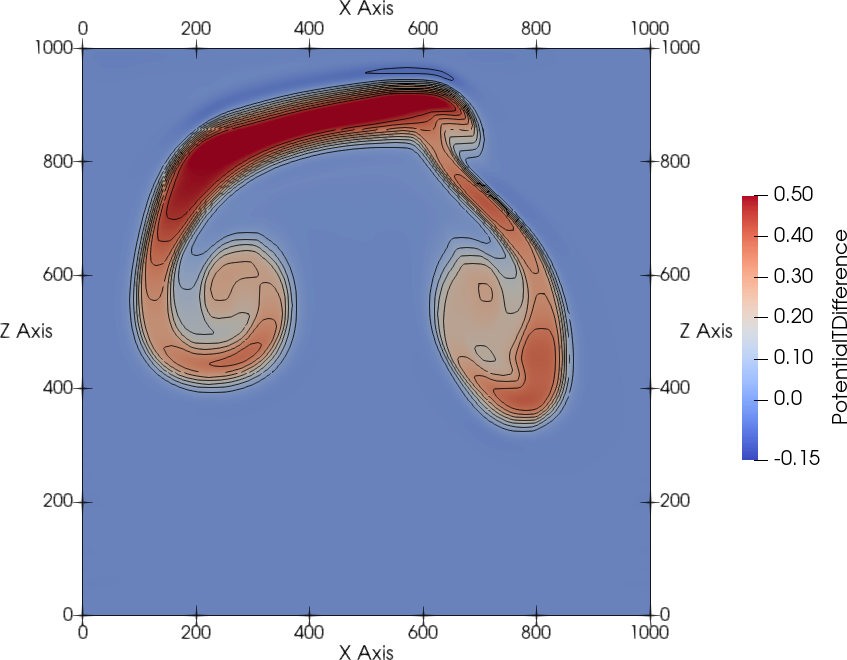
\includegraphics[width=1\textwidth]{screenshots/two_bubbles_fv.png}
  \captionof{figure}{\label{fig:two-bubbles-2d-fv-noamr}%
  2D colliding bubbles scenario, without AMR, computed with Finite Volume method.
  Recomputed and corrected scenario to replace Figure 4 in~\cite{krenz2019high}.%
  }
    \end{minipage}\quad% 
  \begin{minipage}[t]{.473\textwidth}
      \centering 
  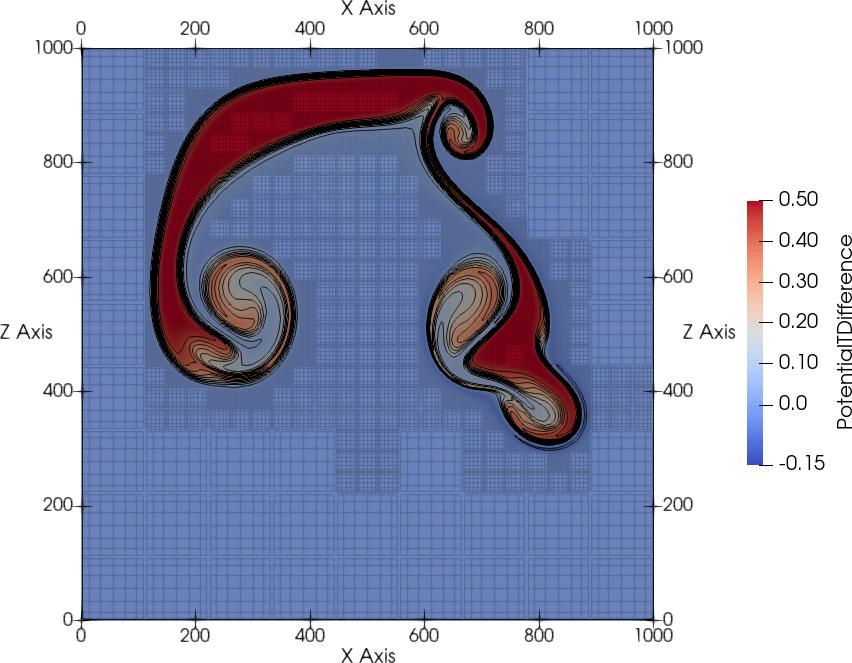
\includegraphics[width=\textwidth]{screenshots/two_bubbles_dg.png}
  \captionof{figure}{\label{fig:two-bubbles-2d-dg-amr}%
  2D colliding bubble with AMR, computed by ADER-DG method.
  Contours are at $-0.05, 0.05, \ldots 0.45$.
  Recomputed and corrected scenario to replace Figure 5 in~\cite{krenz2019high}.%
  }
  \end{minipage}
  \end{figure}

\paragraph{Colliding Bubble (Sec.~4.2. and Fig.~6 of\cite{krenz2019high})}
We ran the colliding bubble scenario with the ADER-DG method and a viscosity of $\mu=0.1$.
Similarly to the cosine bubble, the results with AMR (\cref{fig:two-bubbles-2d-dg-amr}) show a very close agreement with the original results, with some small differences in the refinement.
The simulation with AMR also agrees with our results.
Additionally, we simulated this scenario with the Finite Volume method and a viscosity of $\mu=0$.
The results (\cref{fig:two-bubbles-2d-fv-noamr}) agree with the original results.

%\subsection*{Acknowledgments}
%This work was funded by the European Union’s Horizon 2020 Research and Innovation Programme under grant agreements 
%No~671698 (project ExaHyPE, \url{www.exahype.eu}) and 
%No~823844 (ChEESE centre of excellence, \url{www.cheese-coe.eu}).
%Computing resources were provided by the Leibniz Supercomputing Centre (project pr83no).

\bibliographystyle{CP032_spmpsci}
\bibliography{CP032_bibliography}{}
\end{document}
